\documentclass[11pt]{article}

% ---------------- Packages ----------------
\usepackage[margin=1in]{geometry}
\usepackage{amsmath}
\usepackage{graphicx}
\usepackage{float}
\usepackage{booktabs}
\usepackage{xcolor}
\usepackage{listings}
\usepackage{hyperref}

% ---------------- Figure path ----------------
\graphicspath{{figures/}}

% ---------------- Code formatting ----------------
\lstset{
    basicstyle=\ttfamily\small,
    breaklines=true,
    frame=single,
    keywordstyle=\color{blue},
    commentstyle=\color{gray}
}

% ---------------- Title Info ----------------
\title{LSTM-Based Solar Power Prediction Using Historical and Local Data}
\author{Dominick Choate}
\date{\today}

\begin{document}

\maketitle

% ============================================================
\section{Project Description}

	This project is a continuation and completion of unfinished work that I originally started during an REU (Research Experiences for Undergraduates) program in the summer of 2025. The research was part of the DigiCAREs Project, which focuses on advancing renewable energy studies and smart energy systems. As part of the project, I was tasked by Dr. Fan Guiliang and Dr. Ying Zhang with designing and implementing an LSTM (Long Short-Term Memory) recurrent neural network (RNN) using Python for renewable energy prediction. Over the course of approximately five months, I developed three separate LSTM models for wind, solar, and hybrid renewable energy prediction. The primary focus of this project is the solar LSTM model, since its original performance was significantly weaker than the wind and hybrid models, producing an RMSE of approximately 1801.52. Several factors contributed to the poor performance, including inefficient preprocessing methods, poor feature selection, and limited experience with large-scale machine learning workflows at the time.

	The revised version of the project focuses on redesigning and improving the original neural network pipeline by implementing cubic spline interpolation for missing-data handling, restructuring the dataset split ratios, improving validation methods, and reducing unnecessary variables through feature importance analysis. The original project used a 50/50 training and prediction split, while the revised model now uses a time-ordered 80/10/10 training, validation, and testing split to improve generalization and stability. In addition to the historical solar dataset, the project was expanded to support locally collected solar panel data from the Endeavor system provided by Evan Burk. Unlike the historical dataset, which measured large-scale solar generation in megawatts, the local dataset records minute-level measurements in watts directly from a physical solar power system. This addition allowed the project to move toward short-term local solar forecasting using both environmental and system-state variables while also supporting future live-data integration.

% ============================================================
\section{Numerical Method}

	The numerical method chosen to be implemented into the LSTM project was cubic spline interpolation. This method was selected because of its strong ability to handle missing values within time-series datasets, which is especially important in renewable energy prediction. In the case of solar power generation, missing or low-output values are common due to cloud coverage, poor weather conditions, sensor interruptions, or nighttime periods where solar production naturally drops to zero. Cubic spline interpolation works by estimating intermediate values between known data points using smooth cubic polynomial functions. In simpler cases, the interpolation behaves similarly to estimating values between surrounding points while maintaining a smooth overall curve. This works well for smaller gaps in the dataset, although very large gaps can still introduce inaccuracies because significant environmental changes may occur during those missing periods.

\[
S_i(x)=a_i x^3+b_i x^2+c_i x+d_i
\]

	Each interval between data points receives its own cubic polynomial while also maintaining smooth transitions between neighboring intervals through continuity in the first and second derivatives. In this project, the cubic spline interpolation method was applied before normalization and sequence generation in order to improve the overall preprocessing pipeline and reduce disruptions caused by missing data. By preserving smoother transitions within the solar generation and weather datasets, the interpolation process helped improve continuity in the time-series input data used for LSTM training. This allowed the neural network to learn patterns more effectively without needing to discard large portions of incomplete data.

% ============================================================
\section{Project Goals}

% Writing ideas:
% - Improve original train/prediction split.
% - Add validation phase.
% - Reduce variables while preserving accuracy.
% - Compare against persistence baseline.
% - Add local dataset mode.
% - Add tests and GitHub workflow.
% - Support future live data integration.

Write your project goals here.

% ============================================================
\section{Model Structure}

% Writing ideas:
% - Explain that LSTM is used because the data is time-series.
% - Explain that the model uses previous time steps to predict future power.
% - Explain that historical and local mode use the same general pipeline.
% - Mention that local data uses short-term prediction.

The general model structure is

\[
\text{Past weather/system variables + past power} \rightarrow \text{future power}
\]

Write your model structure explanation here.

% ============================================================
\section{Data Splitting}

% Writing ideas:
% - Explain original version used 50/50 split.
% - Explain why that was a problem.
% - Explain the new 80/10/10 split.
% - Mention that the split is time-ordered, not randomized.
% - Explain that validation is used for early stopping.

The revised project uses a time-ordered split:

\[
80\% \text{ training}, \quad 10\% \text{ validation}, \quad 10\% \text{ testing}
\]

Write your data splitting explanation here.

% ============================================================
\section{Evaluation Metrics}

% Writing ideas:
% - Define RMSE, MAE, and SMAPE.
% - Explain that RMSE is used for same-dataset comparison.
% - Explain historical data and local data are on different scales.
% - Historical data is larger-scale generation, local data is watts.
% - Therefore, RMSE should not be directly compared between datasets.

\[
RMSE = \sqrt{\frac{1}{n}\sum_{i=1}^{n}(y_i-\hat{y}_i)^2}
\]

\[
MAE = \frac{1}{n}\sum_{i=1}^{n}|y_i-\hat{y}_i|
\]

\[
SMAPE = \frac{100}{n}\sum_{i=1}^{n}
\frac{|y_i-\hat{y}_i|}{(|y_i|+|\hat{y}_i|)/2}
\]

Write your evaluation metrics explanation here.

% ============================================================
\section{Historical Dataset Results}

% Writing ideas:
% - Mention original solar LSTM RMSE was 1801.52.
% - Mention revised model was compared against a persistence baseline.
% - Mention feature reduction improved the result.
% - Mention revised historical LSTM beat the persistence baseline based on RMSE.
% - Mention model still underestimates some peak values.

\begin{table}[H]
\centering
\begin{tabular}{lccc}
\toprule
Model & RMSE & MAE & SMAPE \\
\midrule
Original Solar LSTM & 1801.52 & -- & -- \\
Persistence Baseline & 714.43 & 411.59 & 57.85\% \\
Revised Historical LSTM & 659.06 & 291.73 & 56.20\% \\
\bottomrule
\end{tabular}
\caption{Historical dataset model comparison.}
\label{tab:historicalresults}
\end{table}

Write your historical results explanation here.

\begin{figure}[H]
\centering
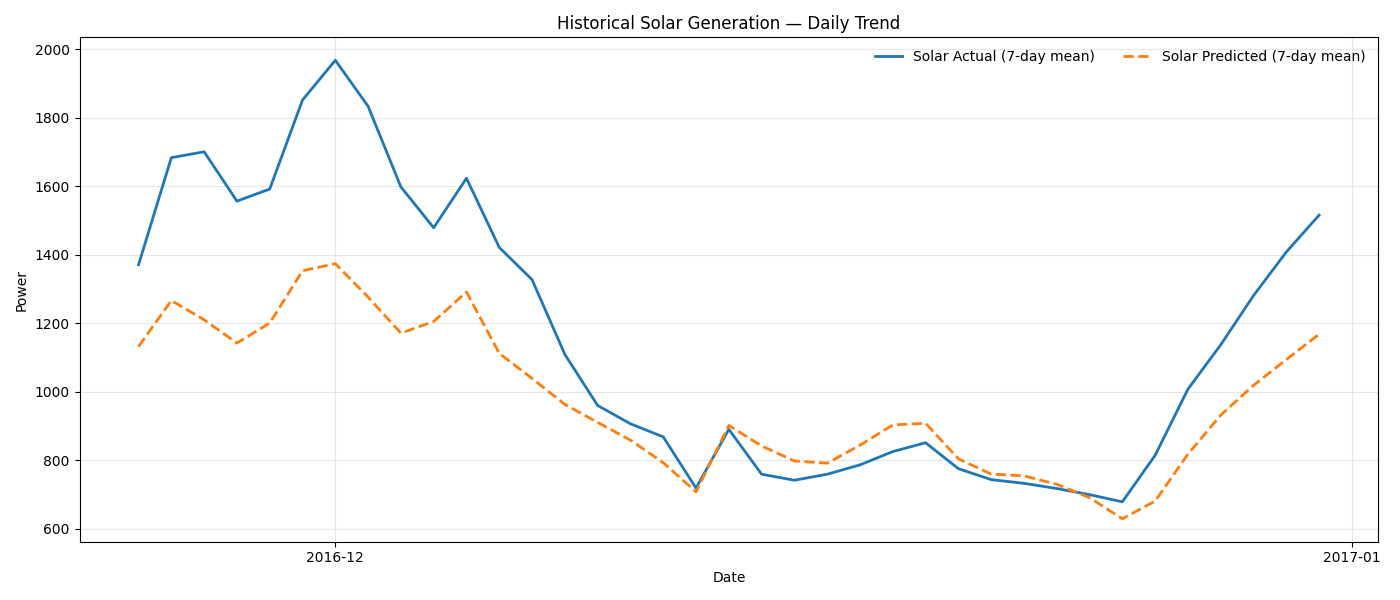
\includegraphics[width=0.95\textwidth]{daily_trend_new.png}
\caption{Historical solar generation compared against the predicted 7-day rolling mean trend.}
\label{fig:historicaltrend}
\end{figure}

% Writing ideas for this figure:
% - The predicted curve follows the same general trend.
% - It underestimates high peaks.
% - It performs better during lower-generation periods.
% - The rolling mean smooths short-term variation.

\begin{figure}[H]
\centering
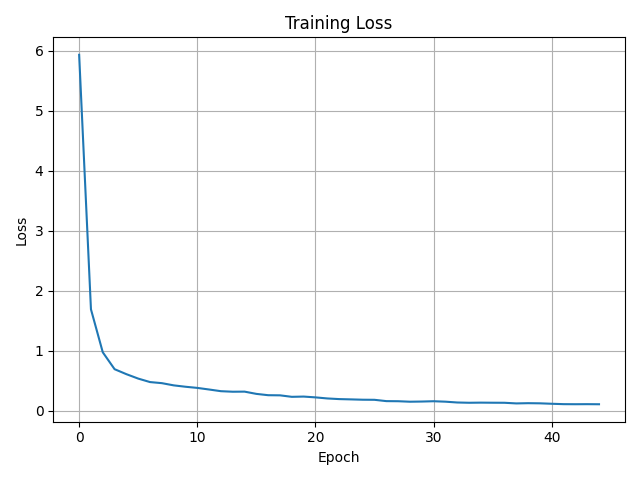
\includegraphics[width=0.75\textwidth]{training_loss_new.png}
\caption{Training loss for the revised historical LSTM model.}
\label{fig:historicaltrainingloss}
\end{figure}

% Writing ideas for this figure:
% - Loss decreases quickly early in training.
% - The model converges without unstable oscillation.
% - Early stopping helps prevent unnecessary training.

% ============================================================
\section{Historical Feature Importance}

% Writing ideas:
% - Explain permutation feature importance.
% - A feature is shuffled and the RMSE change is measured.
% - Larger RMSE increase means more important feature.
% - Negative increase means the feature may hurt performance.
% - Mention SWTDN and SWGDN were most important.
% - Mention dew hurt performance and was a candidate for removal.

\begin{table}[H]
\centering
\begin{tabular}{lc}
\toprule
Feature & RMSE Increase \\
\midrule
SWTDN & 1201.44 \\
SWGDN & 1094.27 \\
Cloud Cover & 144.90 \\
Humidity & 98.52 \\
Dew & -47.69 \\
\bottomrule
\end{tabular}
\caption{Historical permutation feature importance results.}
\label{tab:historicalfeatures}
\end{table}

Write your historical feature importance explanation here.

% ============================================================
\section{Local Dataset Results}

% Writing ideas:
% - Explain local data comes from Endeavor solar system.
% - Explain local data is in watts, unlike historical data.
% - Mention data was recorded approximately every minute.
% - Explain local mode predicts short-term PV power.
% - Mention local mode uses system variables and weather variables.
% - Mention results should be compared to local persistence only.

\begin{table}[H]
\centering
\begin{tabular}{lccc}
\toprule
Model & RMSE & MAE & SMAPE \\
\midrule
Persistence Baseline & -- & -- & -- \\
Local LSTM & 7.18 & -- & -- \\
\bottomrule
\end{tabular}
\caption{Local dataset model comparison. Fill in final persistence values from terminal output.}
\label{tab:localresults}
\end{table}

Write your local results explanation here.

\begin{figure}[H]
\centering
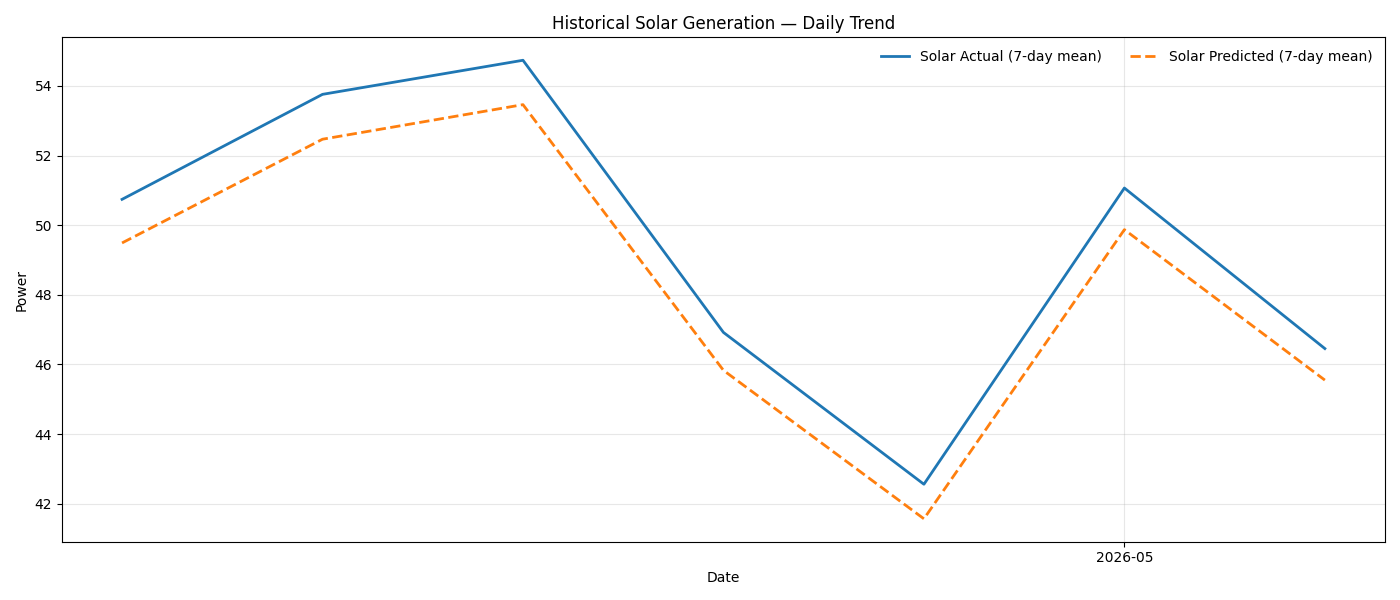
\includegraphics[width=0.95\textwidth]{7_day_trend_local.png}
\caption{Local solar prediction trend using the Endeavor solar dataset.}
\label{fig:localtrend}
\end{figure}

% Writing ideas for this figure:
% - The local prediction follows the actual trend closely.
% - Because the scale is smaller, errors are shown in watts.
% - Nighttime and low-output periods affect the shape of the curve.
% - The local model is more focused on short-term behavior than seasonal behavior.

\begin{figure}[H]
\centering
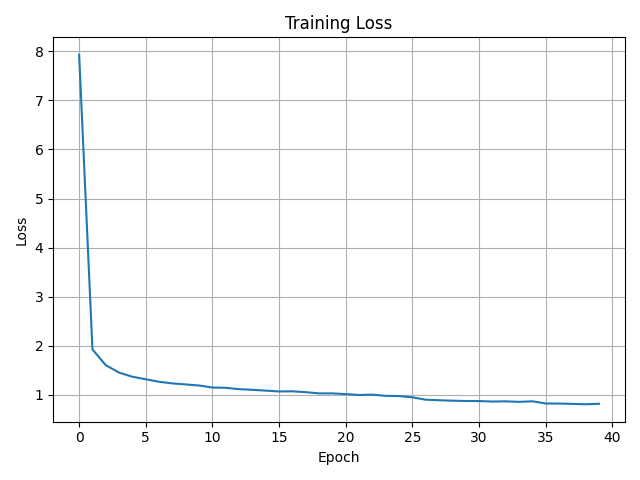
\includegraphics[width=0.75\textwidth]{Training_loss_local.png}
\caption{Training loss for the local solar prediction model.}
\label{fig:localtrainingloss}
\end{figure}

% Writing ideas for this figure:
% - The loss decreases rapidly.
% - This shows the model learned the local system patterns.
% - If there is flattening, that suggests convergence.

% ============================================================
\section{Local Feature Importance}

% Writing ideas:
% - Explain local feature importance showed system variables were strongest.
% - Avg power to battery and battery power were highly important.
% - Solar irradiance was also important.
% - Some weather variables contributed less.
% - Explain this makes sense because local prediction horizon is short.
% - Short-term prediction often depends strongly on recent system state.

\begin{table}[H]
\centering
\begin{tabular}{lc}
\toprule
Feature & RMSE Increase \\
\midrule
Avg Power to Battery & 26.28 \\
Battery Power & 18.93 \\
Solar Irradiance & 11.14 \\
PV Voltage & 9.39 \\
Wind Speed & 0.58 \\
PV Current & 0.57 \\
UV Index & 0.37 \\
Humidity & 0.16 \\
Air Temperature & 0.13 \\
Air Pressure & 0.01 \\
\bottomrule
\end{tabular}
\caption{Local dataset permutation feature importance results.}
\label{tab:localfeatures}
\end{table}

Write your local feature importance explanation here.

% ============================================================
\section{Testing and GitHub Workflow}

% Writing ideas:
% - Mention repository was public.
% - Mention pytest was used for self-tests.
% - Mention GitHub workflow automation.
% - Explain tests verify numerical method, metrics, and model shape.
% - Mention tests passed successfully.

\begin{table}[H]
\centering
\begin{tabular}{ll}
\toprule
Test File & Purpose \\
\midrule
\texttt{test\_basic.py} & Basic pytest sanity check \\
\texttt{test\_metrics.py} & Verifies RMSE calculation \\
\texttt{test\_spline\_interpolation.py} & Verifies cubic spline missing-data handling \\
\texttt{test\_model\_shapes.py} & Verifies LSTM output dimensions \\
\bottomrule
\end{tabular}
\caption{Automated test coverage used in the project.}
\label{tab:tests}
\end{table}

Write your testing and GitHub workflow explanation here.

% ============================================================
\section{Limitations and Future Work}

% Writing ideas:
% - Local data is limited compared to the historical dataset.
% - More local data would improve generalization.
% - True live data integration is still a future step.
% - Weather-only local prediction was weaker than system-state prediction.
% - More forecast horizons should be tested, such as 15, 30, and 60 minutes.

Write your limitations and future work here.

% ============================================================
\section{Conclusion}

% Writing ideas:
% - Summarize that project improved original solar LSTM.
% - Mention original RMSE was 1801.52 and revised historical model improved.
% - Mention cubic spline interpolation was implemented.
% - Mention local mode was added.
% - Mention feature importance helped reduce variables.
% - Mention automated testing was added.
% - End with how this supports future live solar prediction.

Write your conclusion here.

% ============================================================
\end{document}